\subsection{Estimating the point of impact}
Estimating a point of impact. 
One of the main obstacles we faced while programming the Phong shading model, was determining the exact points in world coordinates on which the light hit the box surface. This point is needed for correct visualization of both the diffuse and the specular lighting. As a bad estimate we started out just by using the center point for each surface, but the results gained from this method were not impressive. Instead we tried to utilize that we had some known points on each surface, trying to estimate some points in between to use in a more realistic lighting model. 
Instead of iterating through the pixels of each surface, we iterate through the 10x10 shadeRes matrix. Each point in 2d here corresponds to a 3d point on the box surface. (Note that we also experienced a bit with using a homography from the box surface in 3d to a 2d coordinate system, in effect doing an inverse projection, but instead we decided to estimate it the other way around).
As our 2d coordinate system in this case is 10x10  each surface determines the vector from the center to one of the corner points. This vector is divided by 5 to get the increment factor of each axis. This factor times ten (each axis x,y,z fully incremented) gives us the opposite corner point. Each time we increment either of the axis (x or y) in  our 2d coordinate system, we increment each axis accordingly in our 3d world coordinate system adding the value to our start/corner coordinate, thus allowing us to iterate through each surface on the box. The new light vector is then calculated from the light source to the surface point in world coordinates.

\begin{figure}[H]
    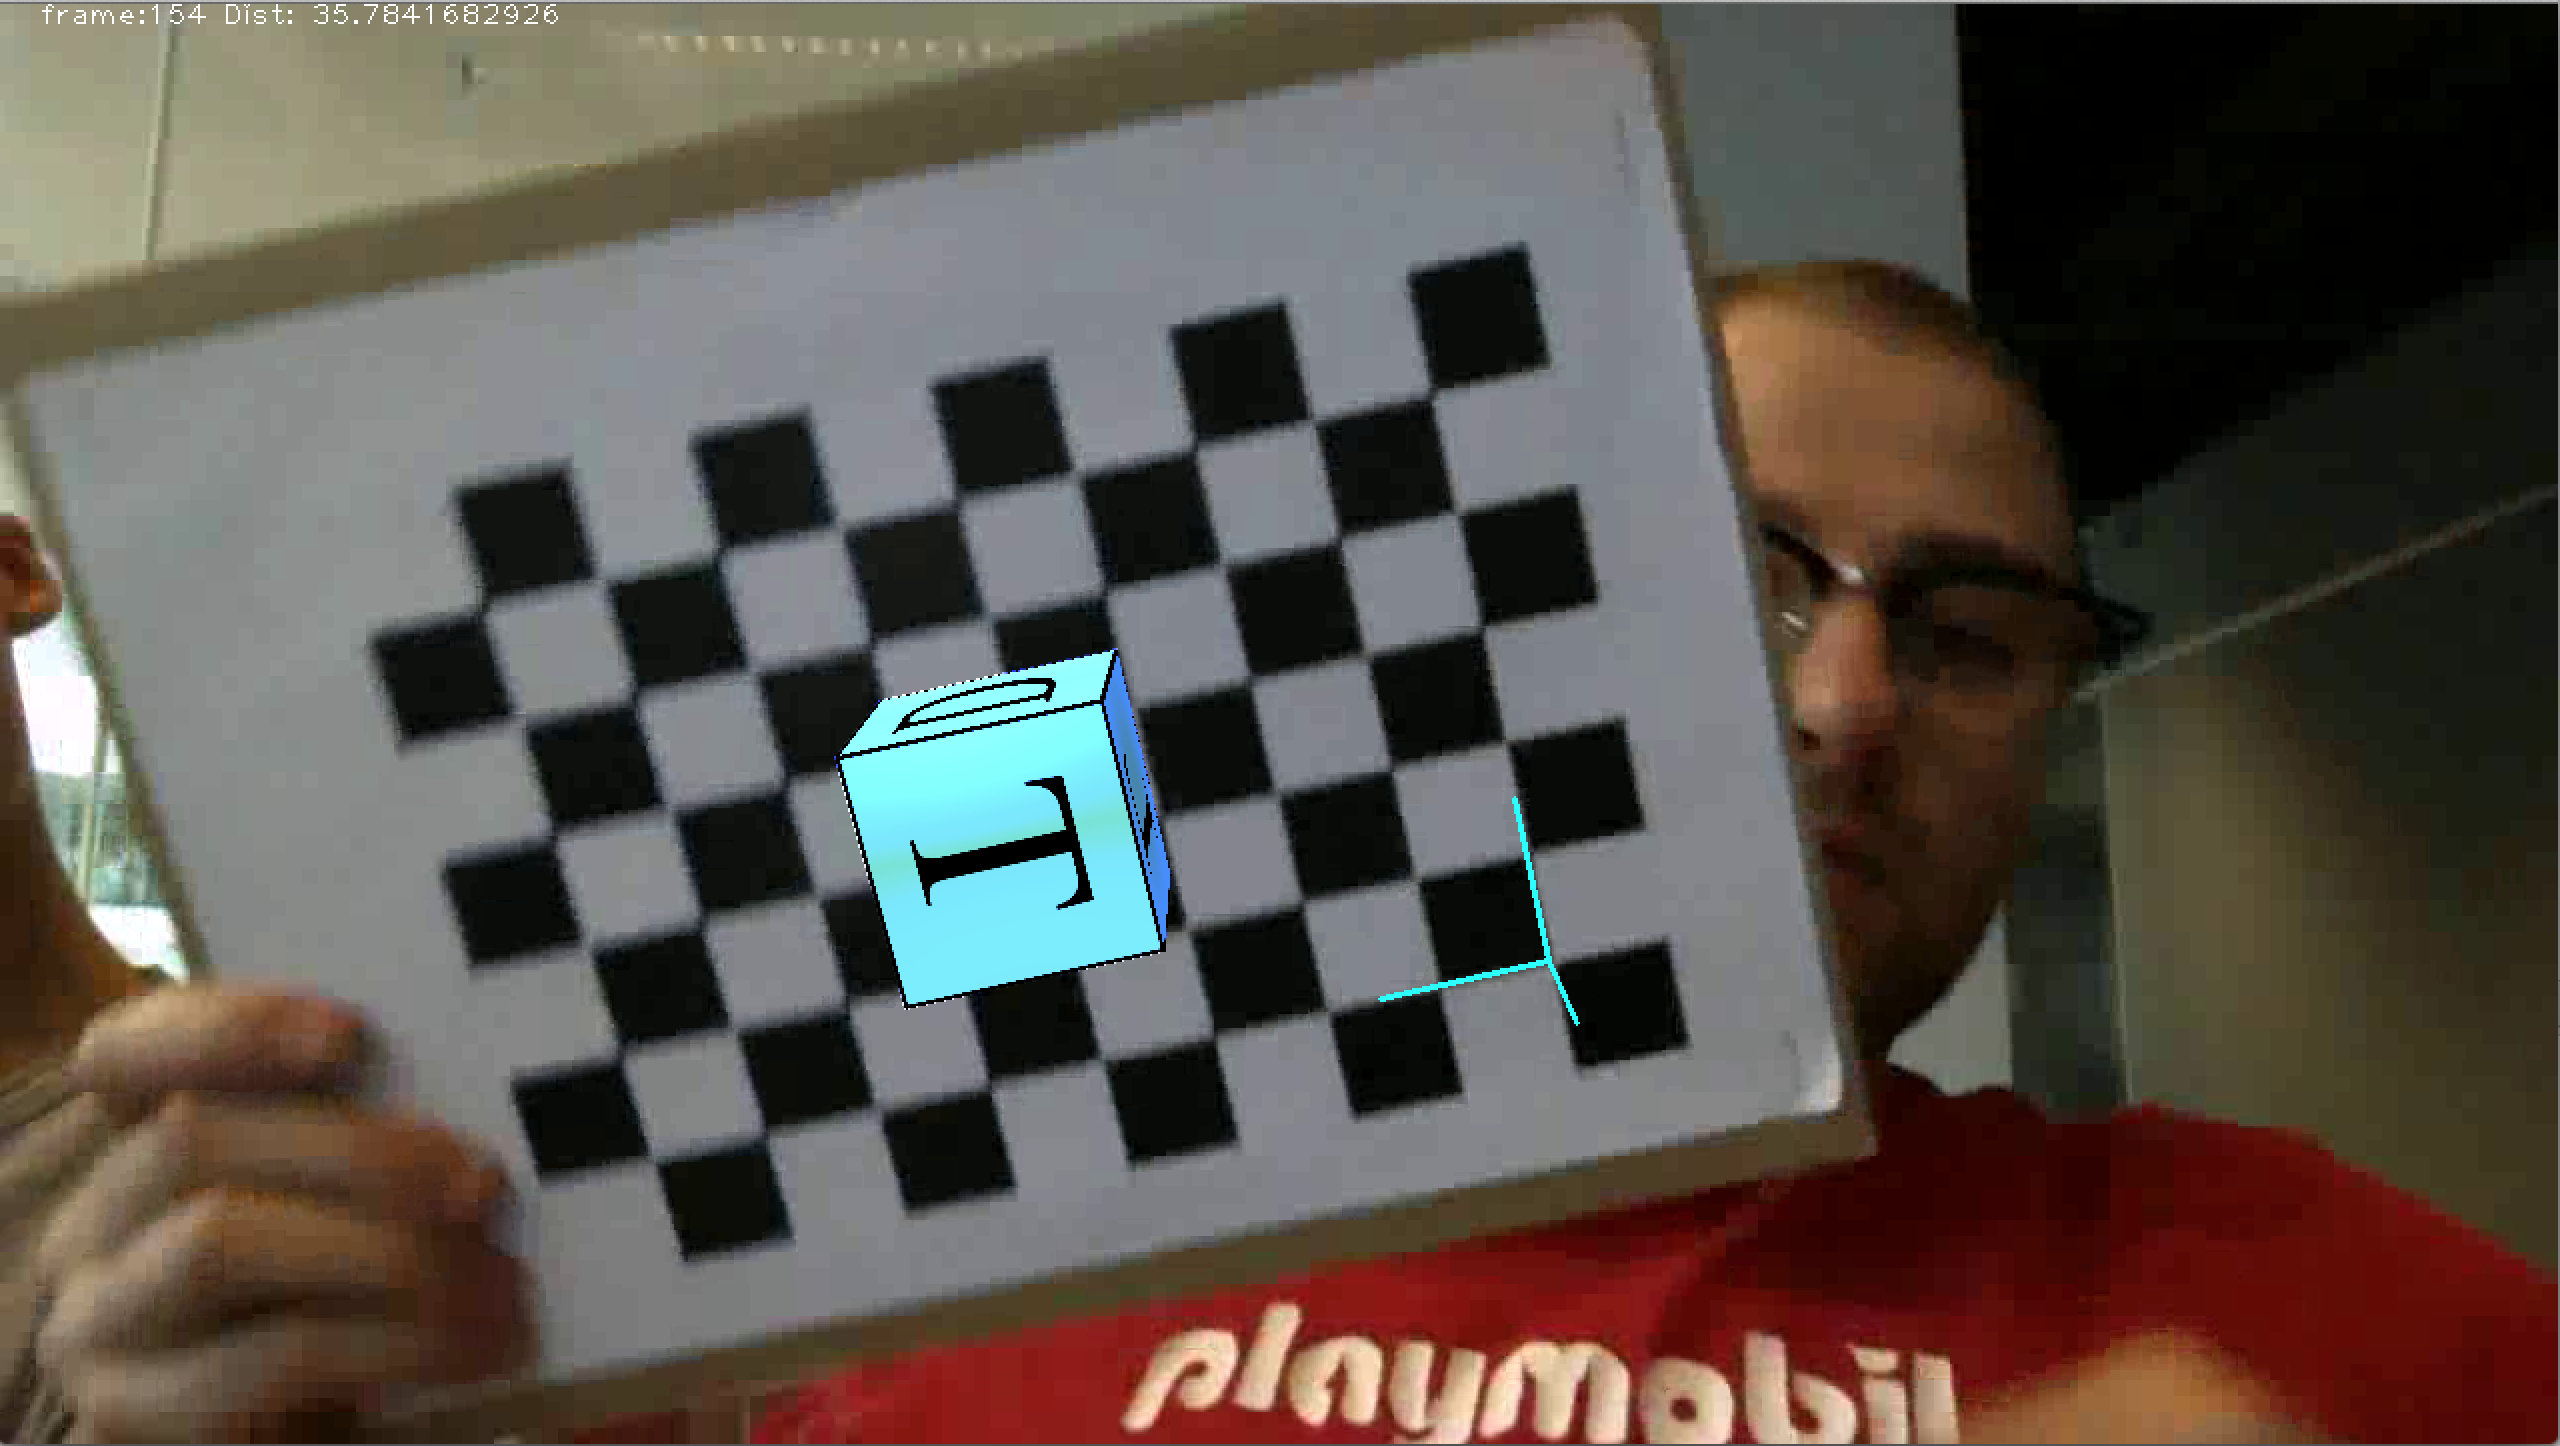
\includegraphics{pics/boxCenterLightVector.png}
    \label{fig:BoxCenter}
    \caption{\textbf{Using the surface center as the impact point of the light for all surface pixels.} Using the box center as the impact point is evidently producing a less satisfying result - not showing much of the specular (white) reflections. This means, that the only effect we get from the added specular lighting to our Phong illumination model is some color changes. The color of the reflectiongs from an object can easily be changed by changing the parameters of the lightsource, but in this case we think its a bug. The color object should ideally not be changed as much as we see in the picture compared to the diffuse-only picture (see below)}
\end{figure}



\begin{figure}[H]
    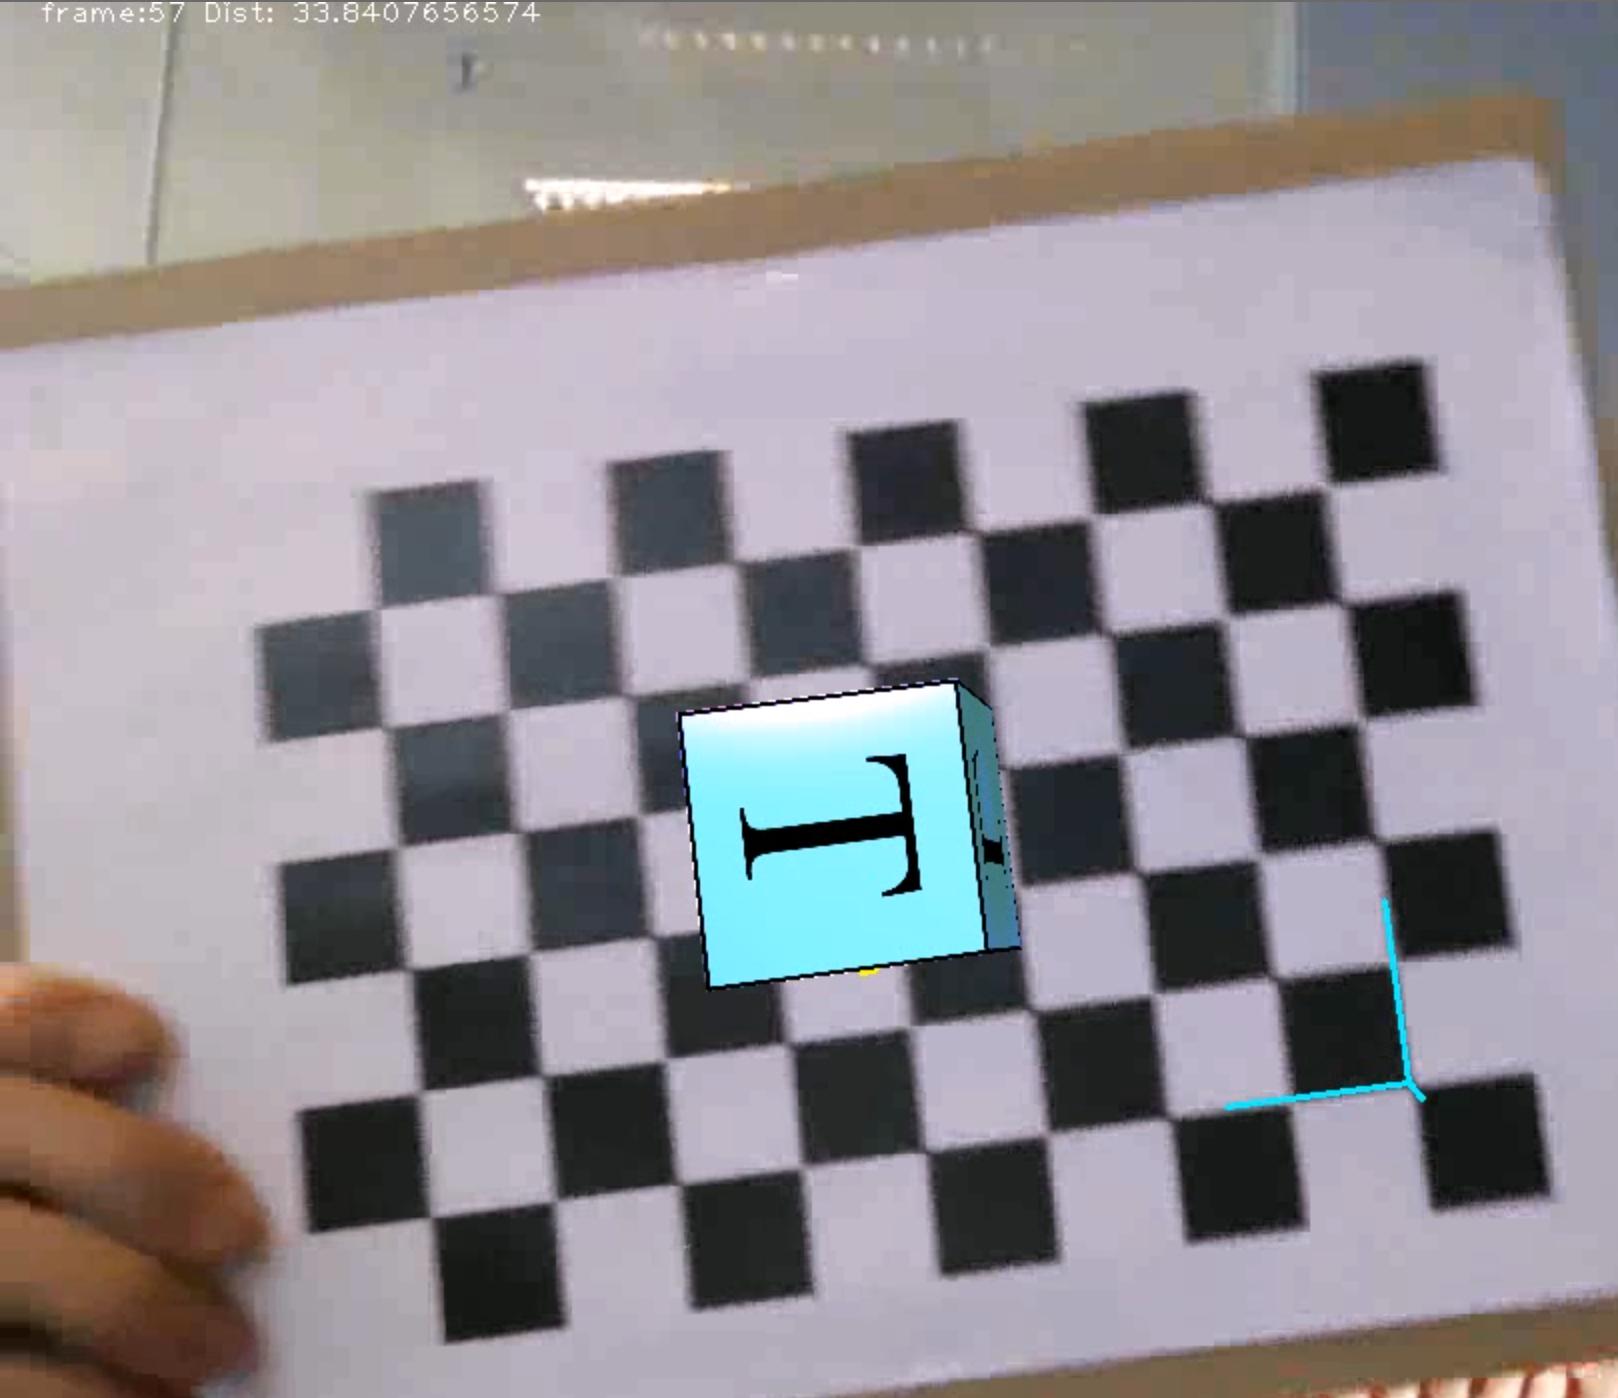
\includegraphics{pics/EstimatedLight.png}
    \label{fig:EstimatedImpactPoint}
    \caption{\textbf{Using our impact point estimation.}}
     The result is better, but far from perfect using our estimated point-of-impact. Getting the correct point in the world coordinates has a huge impact of the realism on the specular lighting, and we're still far from that result. It is an improvement though, over using the surface center as seen in the image above. Some of the specular reflection highlight are shown in with this method, and furthermore shown in the area pointing towards our lightsource. More highlight shine through on surfaces pointing away from our lightsource which is not meant to happen, but we contribute that to two factors:
\begin{itemize}
\item{The estimation contains errors on each surface}
\item{The light source is placed at the camera center, the placement of which is also estimated and not completly reliable.}
\end{itemize}
All in all a result that leave us with a lot of room for improvements.
\end{figure}



\begin{figure}[H]
    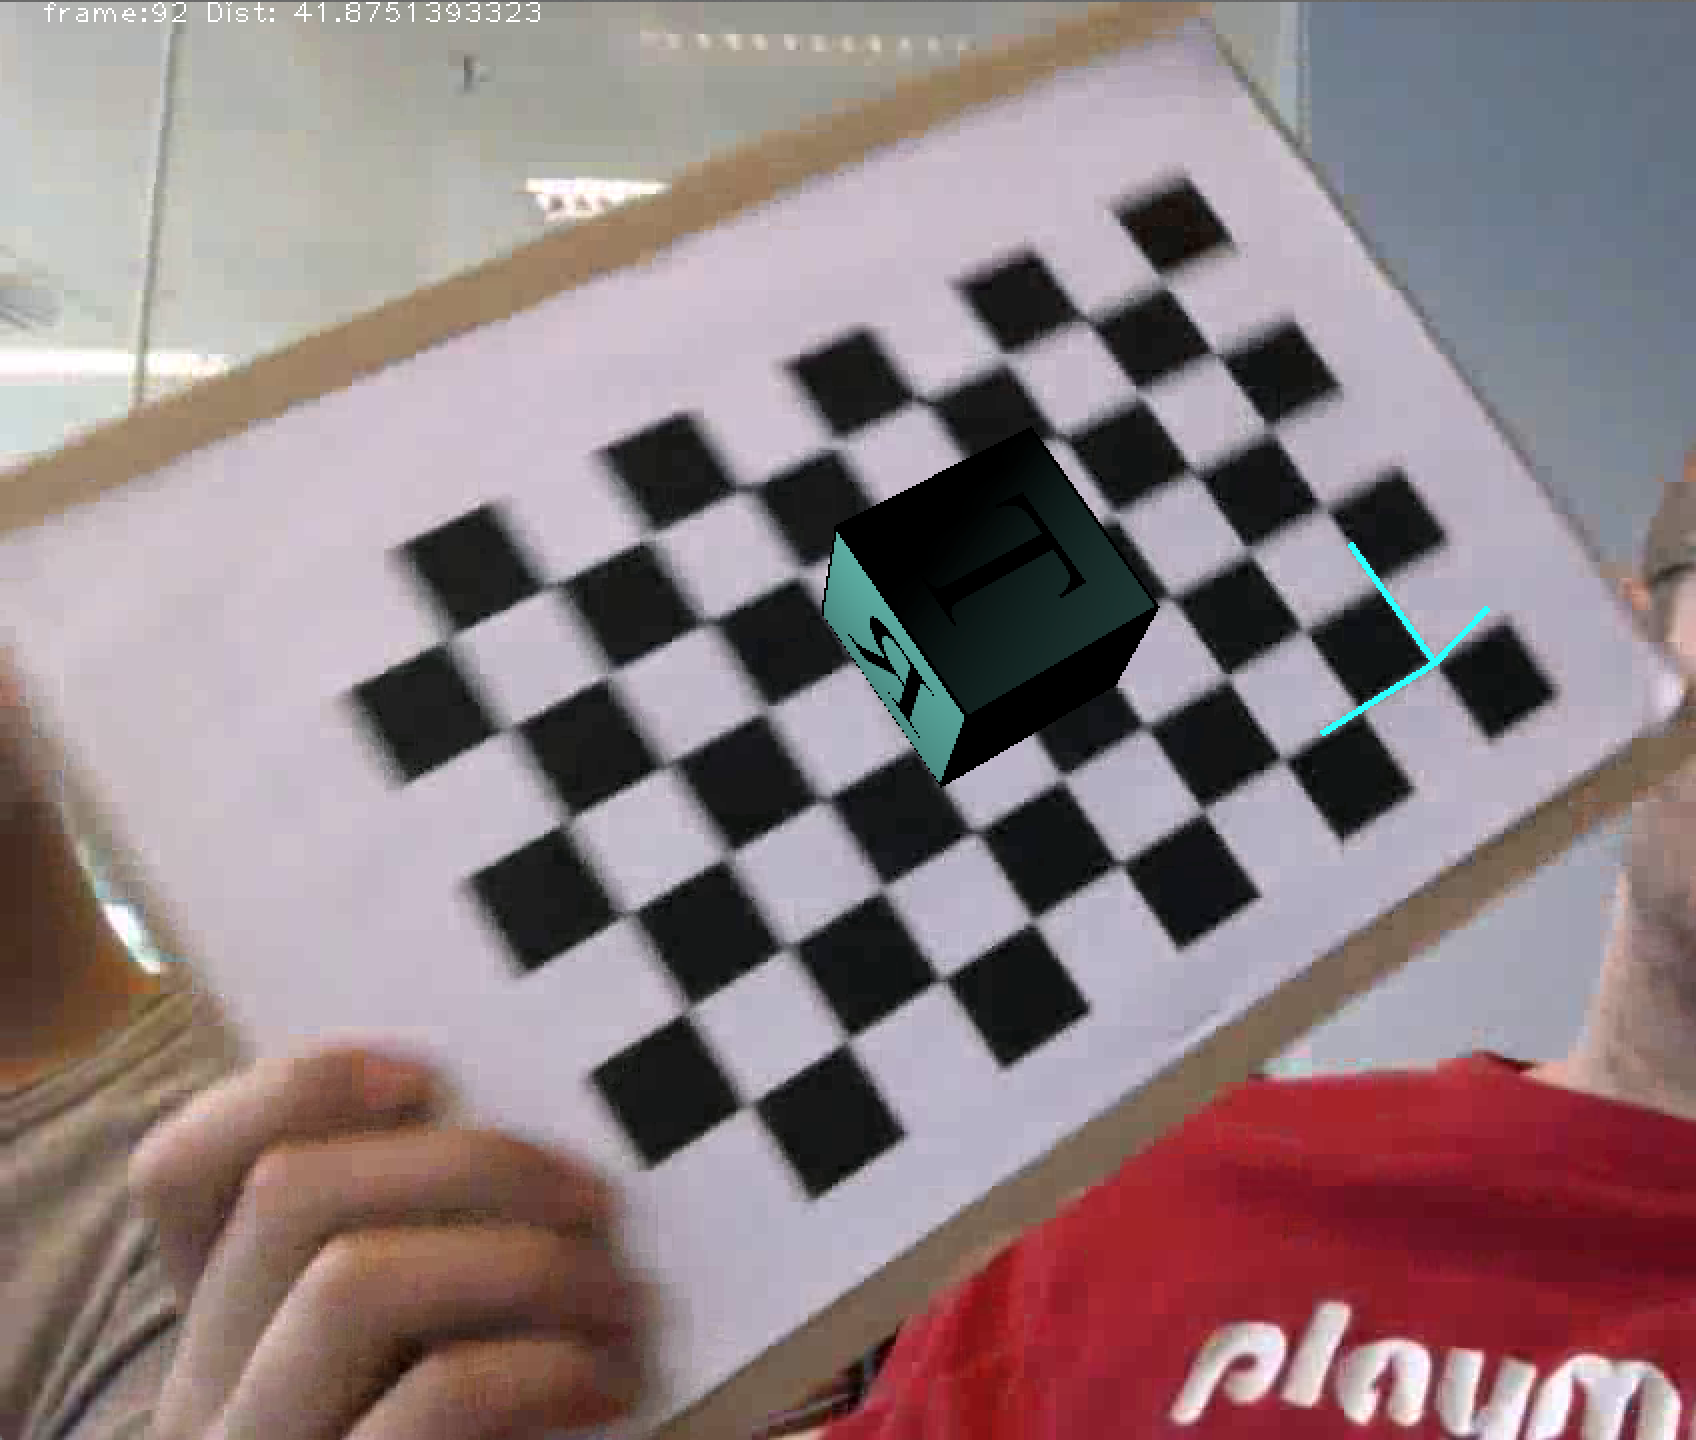
\includegraphics{pics/phongDiffuseOnly.png}
    \label{fig:EphongDiffuseOnly}
    \caption{\textbf{Using phong light model and interpolated shading, but showing diffuse surface light only.} 
    This image shows the color degrading in the other images as the result of the added specular lighting. Note that the result here using only the diffuse light, seems more fitting as it matches the original lighting in the video a bit better. }
\end{figure}
